\documentclass[a4paper, 11pt]{article}
\usepackage{graphicx}
\usepackage[width=160mm, top=25mm, bottom=25mm]{geometry}
\usepackage[utf8]{inputenc}
\usepackage[italian]{babel}
\usepackage{courier}
\usepackage{upgreek}
\usepackage{amsmath}
\usepackage{bm}

\title{\textbf{Misura della caratteristica I-V \\ di due diodi a giunzione p-n}}
\author{Giada Martini \\ Lorenzo Calandra Buonaura}
\date{Turno 3 - 17 Novembre 2022}

\begin{document}

\maketitle

\section{Scopo della prova}
Lo scopo della prova è lo studio delle caratteristiche I-V di due diodi a semiconduttore, uno al silicio (Si) e uno al germanio (Ge). Dopo aver verificato la corretta calibrazione di multimetro e oscilloscopio, sono stati raccolti diversi valori di I e V; dall’analisi dei grafici ottenuti sono stati calcolati i due parametri fondamentali della caratteristica I-V, ossia la corrente inversa $I_0$ e il prodotto $\eta\;V_T$, dove $\eta$ è il fattore di idealità e $V_T$ è l’equivalente in tensione della temperatura. Infine i valori ottenuti sono stati confrontati coi valori attesi.

\section{Schema del circuito}
\begin{figure}[!ht]
  \centering
  \begin{minipage}[b]{0.51\textwidth}
    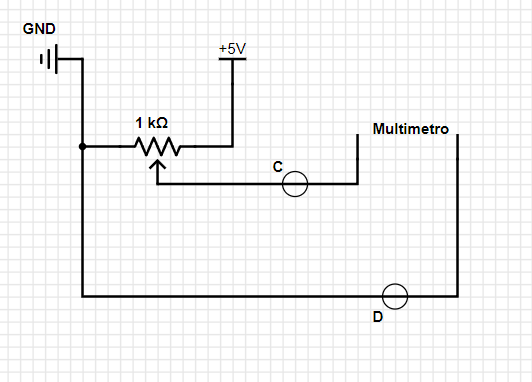
\includegraphics[width=76mm]{LAB _ Circuito senza diodo.png}
    \caption{\textit{Circuito per calibrazione.}}
    \label{fig:Circuitosenzadiodo}
  \end{minipage}
  \hfill
  \begin{minipage}[b]{0.48\textwidth}
    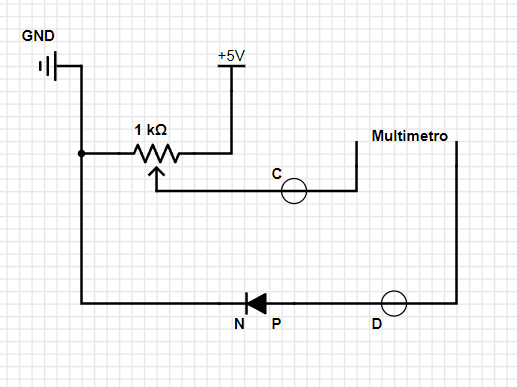
\includegraphics[width=76mm]{LAB _ Circuito con diodo.png}
    \caption{\textit{Circuito con diodo inserito.}}
    \label{fig:Circuito con diodo}
  \end{minipage}
\end{figure}
In Fig.\ref{fig:Circuitosenzadiodo} possiamo vedere il circuito usato per la calibrazione di oscilloscopio e multimetro durante la prima fase dell'esperienza; in questa fase l'oscilloscopio viene collegato nel punto C del circuito. In Fig.\ref{fig:Circuito con diodo}, invece, è stato inserito il diodo (prima Si e poi Ge) fra un capo del multimetro e il GND e in più l'oscilloscopio viene collegato nel punto D: in questo modo è possibile misurare contemporaneamente i valori di corrente e tensione per poi andare a studiare la caratteristica I-V del diodo.

\newpage
\section{Strumenti e materiali utilizzati}
Per l'esperienza sono stati utilizzati i seguenti strumenti e materiali:
\begin{itemize}
    \item Alimentatore di bassa tensione, per fornire il valore del ground di riferiemento e la differenza di potenziale di +5V.
    \item Multimetro digitale, per misurare i valori di corrente.
    \item Oscilloscopio, per misurare i valori di tensione.
    \item Potenziometro da 1 k$\Omega$, in modo da fornire un valore di tensione variabile (fissato con una resistenza pari a R = 500 $\Omega$).
    \item Diodi a giunzione p-n: AAZ15/OA47 Germanio, 1N914A/1N4446/1N4148 Silicio. 
\end{itemize}

\section{Analisi dati}

\subsection{Calibrazione (multimetro ed oscilloscopio)}

\begin{table}[!htb]
    \centering
    \begin{tabular}{|c|c|c|c|c|c|}
    \hline
    \bm{$V_{oscill.} (mV)$} & \bm{$\sigma_{oscill.} (mV)$} &     \bm{$V_{mult.} (mV)$} & \bm{$\sigma_{mult.} (mV)$} & \textbf{\textit{mV/Div}} & \textbf{\textit{Range (V)}} \\
    \hline
    50 & 1.87 &	49 & 0.2 & 10 & 3.200\\ 
    \hline
    80 & 3.16 & 78 & 0.3 & 20 & 3.200\\ 
    \hline
    100 & 3.64 & 98 & 0.4 & 20 & 3.200\\ 
    \hline
    150 & 6.75 & 147 & 0.5 & 50 & 3.200\\ 
    \hline
    200 & 7.83 & 196 & 0.7 & 50 & 3.200\\ 
    \hline
    300 & 13.46 & 297 & 1.0	& 100 & 3.200\\ 
    \hline
    400 & 15.63 & 395 & 1.3	& 100 & 3.200\\ 
    \hline
    500 & 18.03 & 494 & 1.6	& 100 & 3.200\\ 
    \hline
    600 & 26.91 & 592 & 1.9	& 200 & 3.200\\ 
    \hline
    800 & 31.24 & 786 & 2.5	& 200 & 3.200\\ 
    \hline
\end{tabular}
    \caption{Misure di tensione per la calibrazione di multimetro ed oscilloscopio}
    \label{tab:calibrazione}
\end{table}
In Tab.\ref{tab:calibrazione} sono riportati i valori di tensione misurati con oscilloscopio e multimetro per la calibrazione dei due strumenti; sono anche riportati gli errori (per il calcolo vedi \ref{errori}) e il fondo scala utilizzato per ogni misura. Come si può vedere l'errore associato al multimetro risulta trascurabile rispetto a quello associato all'oscilloscopio.

\begin{figure} [!htb]
    \centering
    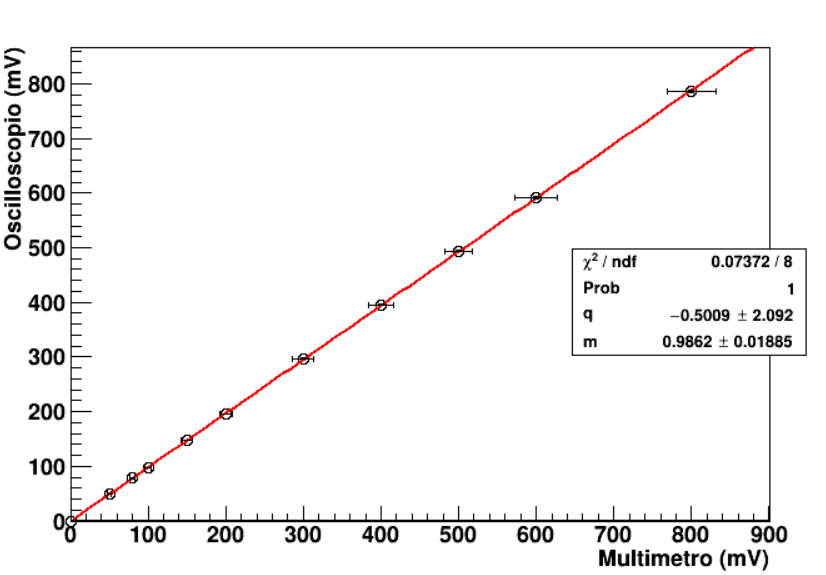
\includegraphics[width = 0.5 \textwidth]{LAB _ Calibrazione.png}
    \caption{Fit lineare per la calibrazione.}
    \label{fig:calibrazione}
\end{figure}
In Fig.\ref{fig:calibrazione} possiamo vedere un grafico che ha sull'asse x i valori di tensione misurati con il multimetro e sull'asse y i valori di tensione misurati contemporaneamente con l'oscilloscopio; in rosso è riportato il fit lineare (\textit{y = mx + q}) per vedere la corretta calibrazione. I valori ottenuti utilizzando ROOT (riportati anche in figura) sono $m = 0.9862 \pm 0.01885$ e $q = -0.5009 \pm 2.092$, compatibili con i valori di corretta calibrazione (ossia $m = 1$ e $q = 0$).

\subsection{Caratteristica I-V dei diodi (Si e Ge)}
\begin{table}[!htb]
    \centering
    \begin{tabular}{|c|c|c|c|c|c|}
        \hline
        \bm{$V_{oscill.} (mV)$} & \bm{$\sigma_{oscill.} (mV)$} &         \bm{$I_{mult.} (mA)$} & \bm{$\sigma_{mult.} (mA)$} & \textbf{\textit{mV/Div}} & \bm{$Range (mA)$} \\
        \hline
        300 & 13.46 & 0.02 & 0.02 & 100 & 32.00\\ 
        \hline
        500 & 18.03 & 0.07 & 0.02 & 100 & 32.00\\ 
        \hline
        560 & 19.56 & 0.19 & 0.02 & 100 & 32.00\\ 
        \hline
        600 & 26.91 & 0.31 & 0.02 & 200 & 32.00\\ 
        \hline
        640 & 27.73 & 0.64 & 0.03 & 200 & 32.00\\ 
        \hline
        660 & 28.15 & 0.90 & 0.03 & 200 & 32.00\\ 
        \hline
        680 & 28.57 & 1.33 & 0.04 & 200 & 32.00\\ 
        \hline
        700 & 29.00 & 1.95 & 0.05 & 200 & 32.00\\ 
        \hline
        720 & 29.44 & 2.73 & 0.06 & 200 & 32.00\\ 
        \hline
        760 & 30.33 & 5.54 & 0.10 & 200 & 32.00\\ 
        \hline
        460 & 17.05 & 0.04 & 0.02 & 100 & 32.00\\ 
        \hline
        520 & 18.54 & 0.12 & 0.02 & 100 & 32.00\\ 
        \hline
        620 & 27.32 & 0.45 & 0.03 & 200 & 32.00\\ 
        \hline
        650 & 27.94 & 0.70 & 0.03 & 200 & 32.00\\ 
        \hline
        800 & 31.24 & 10.04 & 0.17 & 200 & 32.00\\
        \hline
        420 & 16.09 & 0.03 & 0.02 & 100 & 32.00\\ 
        \hline
        480 & 17.54 & 0.06 & 0.02 & 100 & 32.00\\ 
        \hline
    \end{tabular} 
    \caption{Valori di tensione e corrente misurati per il diodo al silicio.}
    \label{tab:silicio}
\end{table}

\begin{table}[!htb]
    \centering
    \begin{tabular}{|c|c|c|c|c|c|}
        \hline
        \bm{$V_{oscill.} (mV)$} & \bm{$\sigma_{oscill.} (mV)$} &         \bm{$I_{mult.} (mA)$} & \bm{$\sigma_{mult.} (mA)$} & \textbf{\textit{mV/Div}} & \bm{$Range (mA)$}
        \\ \hline
        20 & 2.15 & 0.02 & 0.02 & 20 & 32.00\\
        \hline
        64 & 2.82 & 0.02 & 0.02 & 20 & 32.00\\
        \hline
        100 & 5.85 & 0.05 & 0.02 & 50 & 32.00\\
        \hline
        150 & 6.75 & 0.11 & 0.02 & 50 & 32.00\\
        \hline
        180 & 7.38 & 0.18 & 0.02 & 50 & 32.00\\
        \hline
        200 & 7.83 & 0.30 & 0.02 & 50 & 32.00\\
        \hline
        220 & 8.30 & 0.43 & 0.03 & 50 & 32.00\\
        \hline
        240 & 8.78 & 0.63 & 0.03 & 50 & 32.00\\
        \hline
        260 & 12.69 & 0.83 & 0.03 & 100 & 32.00\\
        \hline
        280 & 13.07 & 1.22 & 0.04 & 100 & 32.00\\
        \hline
        300 & 13.46 & 1.76 & 0.05 & 100 & 32.00\\
        \hline
        290 & 13.26 & 1.46 & 0.04 & 100 & 32.00\\
        \hline
        310 & 13.67 & 2.12 & 0.05 & 100 & 32.00\\
        \hline
        320 & 13.87 & 2.41 & 0.06 & 100 & 32.00\\
        \hline
        340 & 14.29 & 3.25 & 0.07 & 100 & 32.00\\
        \hline
        370 & 14.95 & 5.05 & 0.10 & 100 & 32.00\\
        \hline
        75 & 5.51 & 0.03 & 0.02 & 50 & 32.00\\
        \hline
        130 & 6.36 & 0.07 & 0.02 & 50 & 32.00\\
        \hline
    \end{tabular} 
    \caption{Valori di tensione e corrente misurati per il diodo al germanio}
    \label{tab:germanio}
\end{table}

In Tab.\ref{tab:silicio} e in Tab.\ref{tab:germanio} sono riportati i valori di tensione (misurati con l'oscilloscopio) e corrente (misurati con il multimetro) con relativi errori e fondo-scala per i due diodi, rispettivamente al silicio e al germanio. Per il calcolo degli errori vedere Appendice \ref{errori}.

\begin{figure}[!htb]
    \centering
    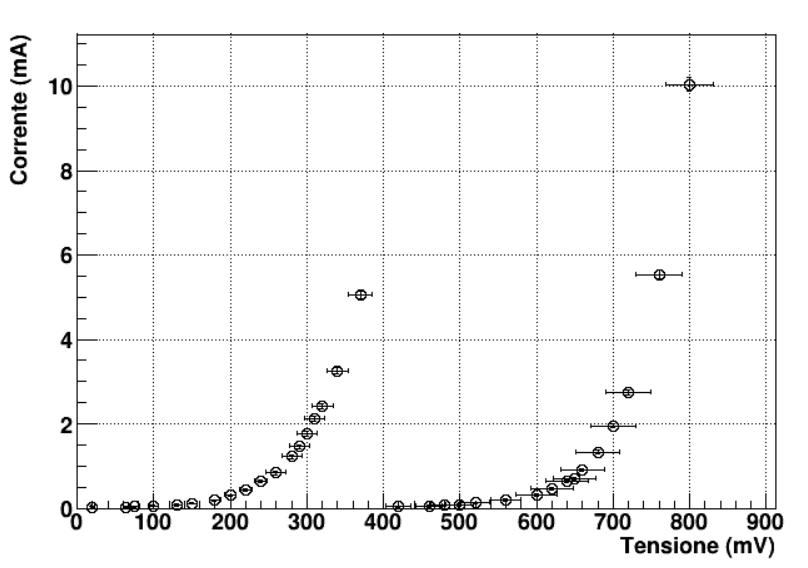
\includegraphics[width = 0.6\textwidth]{LAB _ Grafico totale.png}
    \caption{Grafico di confronto fra le curve caratteristiche I-V dei due diodi utilizzati.}
    \label{fig:graficototale}
\end{figure}

In Fig.\ref{fig:graficototale} possiamo osservare i dati plottati in un grafico: si può notare subito l'andamento esponenziale delle caratteristiche I-V dei due diodi (vedi Appendice \ref{carIV}). \\
Inoltre i valori della tensione di soglia (dopo la quale l'andamento esponenziale prevale) risultano essere qualitativamente compatibili con i valori attesi, rispettivamente di 0.2 V per il germanio e di 0.6 V per il silicio.
\\

\begin{figure}[!htb]
    \centering
    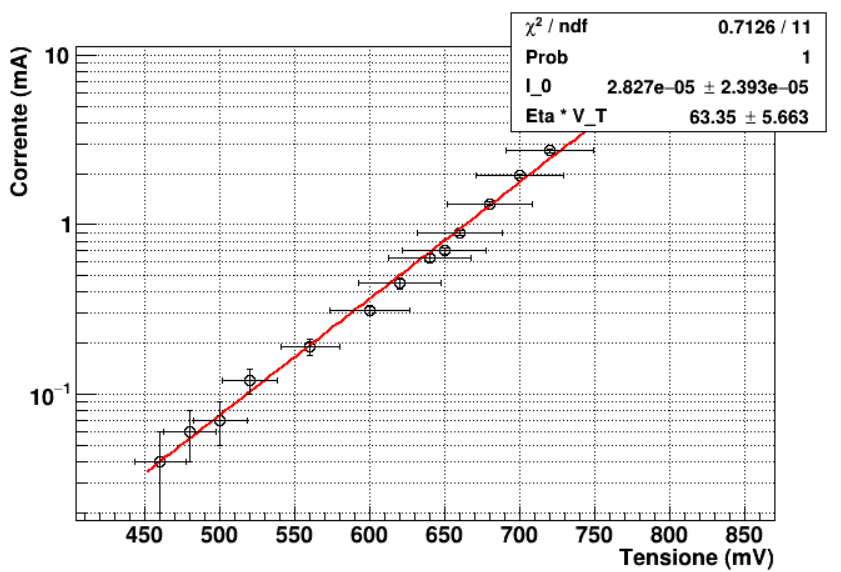
\includegraphics[width = 0.8\textwidth]{LAB _ Fit silicio.png}
    \caption{Caratteristica I-V del diodo al silicio con fit lineare.}
    \label{fig:siliciofit}
\end{figure}

\newpage

\begin{figure}[!htb]
    \centering
    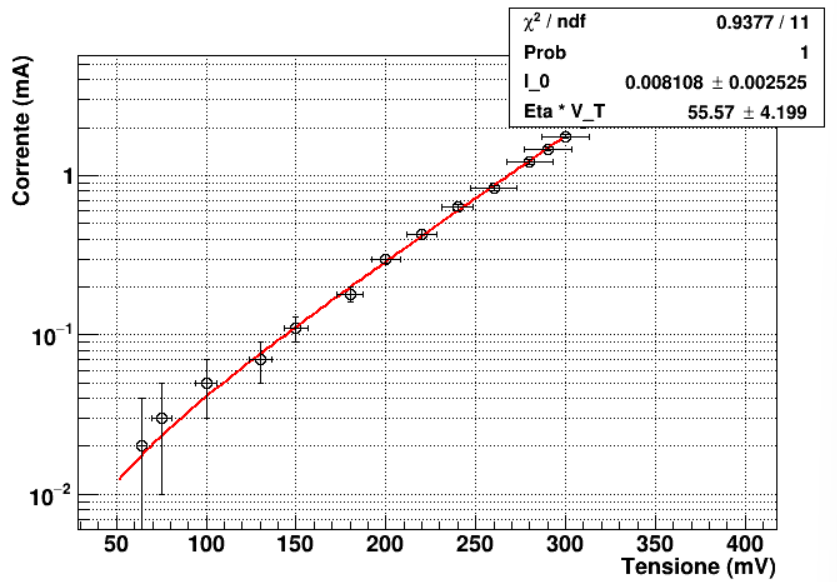
\includegraphics[width = 0.8\textwidth]{LAB _ Fit germanio.png}
    \caption{Caratteristica I-V del diodo al germanio con fit lineare}
    \label{fig:germaniofit}
\end{figure}

In Fig.\ref{fig:siliciofit} e in Fig.\ref{fig:germaniofit} vediamo i dati per i due diodi delle misure di corrente e tensione effettuate; è stato eseguito un fit con la funzione, riportata in Appendice \ref{carIV}, tenendo $I_0$ e $\eta V_T$ come parametri liberi, tramite ROOT (con minimizzazione del Chi Quadro).

Il tutto è stato messo poi in scala semilogaritmica per rendere più evidente il fit nella parte lineare del grafico (che altrimenti risulta schiacciata sullo 0, come si vede in Fig.\ref{fig:graficototale}).
%fit solo in scala semilogaritmica + spiegazione valori attesi/ottenuti%

\section{Risultati finali e conclusioni}
Dalle le caratteristiche I-V dei due diodi, ci aspettiamo che il silicio  abbia una valore di corrente inversa dell'ordine del $nA$ e un prodotto $\eta V_T$ vicino a 50mV poichè $\eta = 2 $, confrontando con qunato ottenuto tramite fit, i parametri ottenuti si avvicinano ai valori attesi.
Infatti, $I_0 = ( 2.827 \pm 2.393) \cdot 10^{-5} mA$ e $\eta V_T = (63.35 \pm 5.66) mV  $.

Per quanto riguarda il germanio, ci aspettiamo che il valore della corrente inversa sia dell'ordine del $\mu A$ e il prodotto $\eta V_T$ vicino a 26mV (a temperatura ambiente T=300K) poichè $\eta = 1$, tuttavia, dai dati estrapolati tramite fit, per quest'ultimo valore, si ottiene una sovrastima del valore atteso, quasi del doppio. Si ha $I_0 = ( 8.10 \pm 2.53) \cdot 10^{-3} mA $ e $\eta V_T = ( 55.57 \pm 4.20) mV$.  

\section{Appendice}

\subsection{Caratteristica I-V di un diodo}
\label{carIV}
La relazione tra corrente (totale) e tensione per un diodo è definita  carratteristica del diodo stesso e segue la relazione:
\begin{equation}
    I(V)=I_0 (e^{\frac{V}{\eta V_T}}-1)
    \label{eq:caratteristica IV}
\end{equation}
dove $I_0$ è definita corrente inversa di saturazione, V  tensione applicata, $\eta$ parametro in funzione del tipo di semiconduttore che si considera ( $\eta = 1 $ per il Ge e $\eta = 2$ per il Si) e $V_T$ è l'equivalente in volt della temperatura.
\subsection{Calcolo degli errori}
\label{errori}
\subsubsection{Oscilloscopio}
L'errore da assocciare ad una misura effettuata con l'oscilloscopio può essere:
\begin{enumerate}
    \item $\sigma = \sqrt{(\sigma_L)^2 + (\sigma_Z)^2 + (\sigma_C)^2}$ nel caso in cui gli errori siano tutti indipendenti;
    \item  $\sigma = \sqrt{(\sigma_L + \sigma_Z)^2 + (\sigma_C)^2}$ nel caso in cui $\sigma_L$ e $\sigma_Z$ siano dipendenti
    \end{enumerate}
dove $\sigma_L$ è l'errore sulla lettura, $\sigma_Z$ è l'errore sullo zero e $\sigma_C$ è l'errore sul costruttore. 

Per quanto riguarda il caso in esame si è utilizzata la prima relazione in quanto errori indipendenti.

Si è calcolato $\sigma_L$ e $\sigma_Z$
secondo la relazione: 
\begin{equation*}
    \sigma = \frac{fondo scala}{5} \cdot ( \# tacchette apprezzabili)
\end{equation*}
Mentre l'errore sul costruttore è del 3\% quindi $\sigma_C = misura \cdot 0.03$.

\subsubsection{Multimetro}

\end{document}
